\documentclass[../../Apputni Fisica.tex]{subfiles}
\begin{document}
Si consideri la figura di seguito riportata.
\begin{figure}[!h]
    \centering
    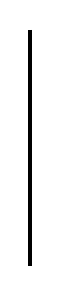
\begin{tikzpicture}[scale = 1, every node/.style={scale=1}]
        \draw [ultra thick] (0, 0) -- (0, -3);

        % TODO: Complete figure.
    \end{tikzpicture}
    \caption{Bussole soggette al campo magnetico di un filo percorso da corrente.}
    \label{fig:18}
\end{figure}

Supponendo di fornire corrente al filo, si osserva che il campo magnetico a distanza \(r\) è paria a
\[
    \oint{}{}{\va{B} \cdot}{\va{s}} = \va{B} \oint{}{}{}{\va{s}} = \frac{\mu_{0} I}{2 \pi r} (2 \pi r) = \mu_{0}I
\]
Quanto detto viene generalizzato dalla \textit{legge di Ampere}, si seguito riportata.
\begin{Law*}[di Ampere]
    L'integrale di \(\va{B} \cdot \dd\va{s}\) su una qualsiasi linea chiusa è pari a \(\mu_{0}I\).
\end{Law*}
\end{document}

